%%% Template originaly created by Karol Kozioł (mail@karol-koziol.net) and modified for ShareLaTeX use

\documentclass[a4paper,11pt]{article}

\usepackage[T1]{fontenc}
\usepackage[utf8]{inputenc}
\usepackage{graphicx}
\usepackage{xcolor}

\renewcommand\familydefault{\sfdefault}
\usepackage{tgheros}
\usepackage[defaultmono]{droidmono}

\usepackage{amsmath,amssymb,amsthm,textcomp}
\usepackage{enumerate}
\usepackage{multicol}
\usepackage{tikz}

\usepackage{geometry}
\geometry{left=25mm,right=25mm,%
bindingoffset=0mm, top=20mm,bottom=20mm}


\linespread{1.3}

\newcommand{\linia}{\rule{\linewidth}{0.5pt}}

% custom theorems if needed
\newtheoremstyle{mytheor}
    {1ex}{1ex}{\normalfont}{0pt}{\scshape}{.}{1ex}
    {{\thmname{#1 }}{\thmnumber{#2}}{\thmnote{ (#3)}}}

\theoremstyle{mytheor}
\newtheorem{defi}{Definition}

% my own titles
\makeatletter
\renewcommand{\maketitle}{
\begin{center}
\vspace{2ex}
{\huge \textsc{\@title}}
\vspace{1ex}
\\
\linia\\
\@author \hfill \@date
\vspace{4ex}
\end{center}
}
\makeatother
%%%

% custom footers and headers
\usepackage{fancyhdr}
\pagestyle{fancy}
\lhead{}
\chead{}
\rhead{}
\lfoot{Object Tracking}
\cfoot{}
\rfoot{Page \thepage}
\renewcommand{\headrulewidth}{0pt}
\renewcommand{\footrulewidth}{0pt}
%

% code listing settings
\usepackage{listings}
\lstset{
    language=Matlab,
    basicstyle=\ttfamily\small,
    aboveskip={1.0\baselineskip},
    belowskip={1.0\baselineskip},
    columns=fixed,
    extendedchars=true,
    breaklines=true,
    tabsize=4,
    prebreak=\raisebox{0ex}[0ex][0ex]{\ensuremath{\hookleftarrow}},
    frame=lines,
    showtabs=false,
    showspaces=false,
    showstringspaces=false,
    keywordstyle=\color[rgb]{0.627,0.126,0.941},
    commentstyle=\color[rgb]{0.133,0.545,0.133},
    stringstyle=\color[rgb]{01,0,0},
    % numbers=left,
    % numberstyle=\small,
    % stepnumber=1,
    % numbersep=10pt,
    % captionpos=t,
    escapeinside={\%*}{*)}
}

%%%----------%%%----------%%%----------%%%----------%%%

\begin{document}

\title{The Extended Kalman Filter}

\author{Mehdi Raza Khorasani, Habib University}

\date{26/6/2021}

\maketitle

\section*{Introduction}
The extended Kalman Filter is an extension to the Kalman Filter Algorithm. The KF algorithm is defined for Discrete time Linear time invariant systems (DT LTI), which are of the form: 
\begin{equation}
    x_k = Fx_{k-1} + V_k 
\end{equation}
\begin{equation}
    y_k = Hx_{k} + W_k 
\end{equation}
The algorithm fails when the system cannot be represented as $(1)$ and $(2)$. The extended KF approach suggests that we linearize the system and obtain a linear approximation, and then develop a KF algorithm for it. The following lines describe how a non linear system can be linearized and a KF algorithm can be applied to it.
\subsection*{The discrete time non-linear system}
Consider a non-linear system, defined by the following equations: 
\begin{equation}
    x_k = f(x_k) + V_k 
\end{equation}
\begin{equation}
    y_k = h(x_{k}) + W_k
\end{equation}
where, $V_k$ and $W_k$ is white uncorrelated Gaussian noise defined as follows: 

\begin{equation*}
    V_k \sim (0, Q_k)
\end{equation*}
\begin{equation*}
    W_k \sim (0, R_k)
\end{equation*}

\section*{The EKF Algorithm}
The algorithm of the EKF consists of linearlizing the plant about the optimal value and consecutively applying the baysian estimation steps. Similarly, the observations are also linearized about the optimal value. The following lines summarize the filtering algorithm: 

\begin{enumerate}
    \item 
    Linearization: Compute the Jacobian of $f$ at $\hat{x}_{k-1|k-1}$ i.e. about the last optimal estimate of $x_k$:
    \begin{equation*}
        F_k = \nabla_{X^T} f(x) \mid_{x = \hat{x}_{k-1|k-1}}
    \end{equation*}
    
    \item 
    State Prediction: Compute Predicted mean and co-variance matrix: 
    \begin{equation*}
        \hat{x}_{k|k-1} = f(\hat{x}_{k-1|k-1})
    \end{equation*}
    \begin{equation*}
        P_{k|k-1} = F_k P_{k-1|k-1} F_k^T + Q_k
    \end{equation*}
    
    \item 
    Linearization: Compute the jacobian of $h$ at $\hat{x}_{k|k-1}$ i.e. about the estimate of $x$ given the last estimate: 
    \begin{equation*}
        H_k = \nabla_{X^T} h(x) \mid_{x = \hat{x}_{k|k-1}}
    \end{equation*}
    
    \item 
    Measurement Prediction: Compute predicted mean, covariance and Kalman gain: 
    \begin{equation*}
        \hat{y}_{k|k-1}  = h(\hat{x}_{k|k-1})
    \end{equation*}
    \begin{equation*}
        S_k = H_k P_{k|k-1} H_k^T + R_k 
    \end{equation*}
    \begin{equation*}
        K_k = P_{k|k-1} H_k^T S_k^{-1}
    \end{equation*}
    
    \item
    Estimation: Compute the posterior mean and co-variance as follows: 
    \begin{equation*}
        \hat{x}_{k|k} = \hat{x}_{k|k-1} + K_k(y_k - \hat{y}_{k|k-1})
    \end{equation*}
    \begin{equation*}
        P_{k|k} = P_{k|k-1} - K_k H_k P_{k|k-1}
    \end{equation*}
\end{enumerate}

\section*{Simulation}
We simulate the non-linear system observed by a Radar. The system and radar are governed by the following equations: 

\begin{equation}
    \boldsymbol{x_k} = 
    \begin{bmatrix}
    x_k\\
    y_k\\
    \phi_k
    \end{bmatrix} = 
    \begin{bmatrix}
    x_{k-1} + T v_k cos(\phi_{k-1}) \\
    y_{k-1} + T v_k sin(\phi_{k-1}) \\
    \phi_{k-1} + T\omega_k
    \end{bmatrix} + 
    \begin{bmatrix}
    V_{1, k}\\
    V_{2, k}\\
    V_{3, k}
    \end{bmatrix}
\end{equation}
\begin{equation}
    \boldsymbol{y_k} = 
    \begin{bmatrix}
    \sqrt{x_k^2+y_k^2}\\
    tan^{-1}\frac{y_k}{x_k}
    \end{bmatrix}
\end{equation}
where $v_k$, $\omega_k$ are the linear and angular velocities of the object respectively and $T$ is sampling time. They are taken as constants: 
\begin{equation*}
    v_k = 0.1, \\ \omega_k = 0.01, \\ T = 0.05
\end{equation*}
\subsection*{Algorithm}

\subsubsection{Initialization}
\begin{enumerate}
    \item 
    The co-variance Matrix of process Noise was taken as follows: 
\begin{equation*}
    Q_k = 
    \begin{bmatrix}
    1e^{-6} & 0 & 0\\
    0 & 1e^{-6} & 0 \\
    0 & 0 & 1e^{-6}
    \end{bmatrix}
\end{equation*}

    \item The co-variance Matrix of Radar Noise was taken as follows: 
\begin{equation*}
    R_k = 
    \begin{bmatrix}
    1e^{-4} & 0 & 0\\
    0 & 1e^{-4} & 0 \\
    0 & 0 & 1e^{-4}
    \end{bmatrix}
\end{equation*}
    
    \item 
    $\mathbf{MATLAB}$'s $randn()$ function was used to generate the the noise vectors $V_k$ and $W_k$ of dimensions $3\times 1$ and $2 \times 1$ respectively.  

    \item 
    Compute the true value of $x_k$ and $y_k$ from the model's equation (5) and (6) to simulate the non-linear object and Radar.
    
\end{enumerate}

\subsubsection{Linearization}
\begin{enumerate}
    \item 
    The pseudo function for this step is as follows: 
    \begin{lstlisting}
        F_k = F_jacobian(T, vk, xhat_km1)
    \end{lstlisting}
    
    \item The jacobian of $f$ is computed as follows: 
    \begin{equation*}
         F_k = \begin{bmatrix}
         \frac{\partial f_1}{\partial x_k} & \frac{\partial f_1}{\partial y_k} & \frac{\partial f_1}{\partial \phi_k} \\ 
         \frac{\partial f_2}{\partial x_k} & \frac{\partial f_2}{\partial y_k} & \frac{\partial f_2}{\partial \phi_k} \\ 
         \frac{\partial f_3}{\partial x_k} & \frac{\partial f_3}{\partial y_k} & \frac{\partial f_3}{\partial \phi_k}
         \end{bmatrix}_{\mathbf{x} = \hat{x}_{k-1|k-1}}
    \end{equation*}
    where: 
    \begin{equation*}
        \begin{bmatrix}
            f_1 \\
            f_2 \\
            f_3 
        \end{bmatrix}
        = 
        \begin{bmatrix}
            x_{k-1} + Tv_k \cos(\phi_{k-1})\\
             y_{k-1} + Tv_k \sin(\phi_{k-1})\\
             \phi_{k-1} + Tw_k 
        \end{bmatrix}_{\mathbf{x} = \hat{x}_{k-1|k-1}}
    \end{equation*}
    
     substituting values and taking respective partial derivatives, we get: 
    \begin{equation*}
         F_k = \begin{bmatrix}
         1 & 0 & -Tv_k \sin{\phi_{k-1}} \\ 
         0 & 1 & Tv_k \cos{\phi_{k-1}} \\ 
         0 & 0 & 1
         \end{bmatrix}_{\mathbf{x} = \hat{x}_{k-1|k-1}}
    \end{equation*}
\end{enumerate}

\subsubsection{State Prediction}
\begin{enumerate}
    \item 
    Pseudo function for this step is: 
     \begin{lstlisting}
        [xhat_predict, P_predict] = state_predict(xhat_km1, P_km1, F_k,  Q_k, vk, wk, T)
    \end{lstlisting}
    \item The mean is predicted by substituting $\hat{x}_{k-1|k-1}$ directly in $f$ of equation (5)
    \item The co-variance is predicted as described earlier.
    
\end{enumerate}

\subsubsection{Linearization}
\begin{enumerate}
    \item 
    The pseudo function for this step is as follows: 
    \begin{lstlisting}
        H_k = H_jacobian(xhat_predict)
    \end{lstlisting}
    
    \item The jacobian of $h$ is computed similar to what was described earlier. It comes out to be:
    \begin{equation*}
         H_k = \begin{bmatrix}
         -\frac{x_k}{\sqrt{x_k^2+y_k^2} } & \frac{x_k}{\sqrt{x_k^2+y_k^2} } & 0 \\ 
         \frac{-y_k}{x_k^2+y_k^2} & \frac{x_k}{x_k^2+y_k^2} & 0 
         \end{bmatrix}_{\mathbf{x} = \hat{x}_{k|k-1}}
    \end{equation*}
\end{enumerate}

\subsubsection{Measurement Prediction}

    The pseudo function for this step is as follows: 
    \begin{lstlisting}
        [yhat_last,K_k] = measurement_predict(xhat_predict, H_k, P_predict, R_k)
    \end{lstlisting}
    
\subsubsection{Estimation}
    The pseudo function for this step is as follows: 
    \begin{lstlisting}
        [xhat_optimal,P_optimal] = estimate(y_k, yhat_predict, P_predict, H_k, K_k)
    \end{lstlisting}

\subsection*{Results}
The true trajectory, sensor observations and predicted trajectory are plotted in figure 1. As can be observed, the EKF algorithm is able to rightly and accurately able to localize the non-linear object. 
\begin{figure}[h]
    \centering
    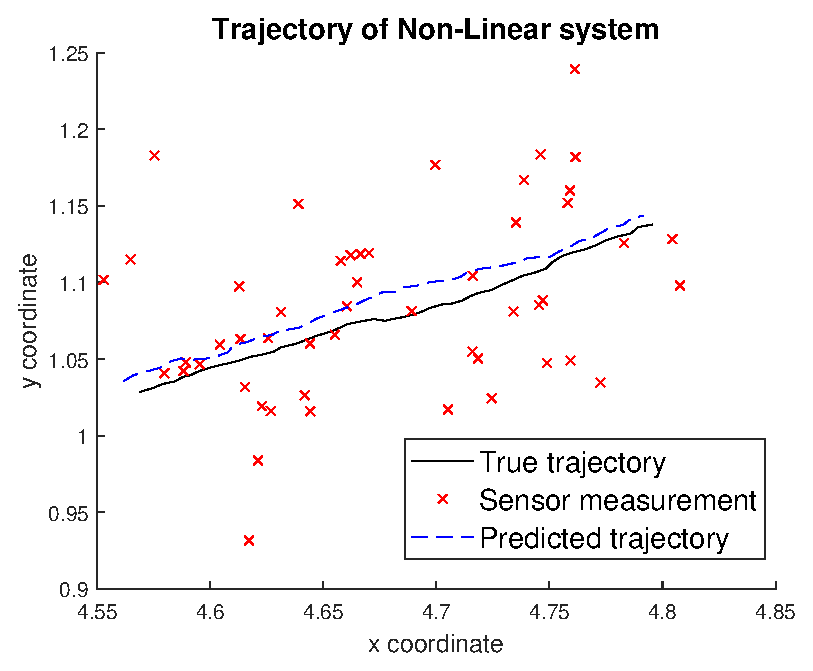
\includegraphics[scale = 1.0]{results.eps}
    \caption{Trajectory of Non linear Object}
    \label{fig:my_label}
\end{figure}

\end{document}
